\chapter{Proposed solution}
\paragraph{}
We have picked SQM as the base for our algorithm. The main factors in this decision were that SQM is faster, produces smaller number of triangles, has better edge flow and even without smoothing the generated mesh better resembles the input skeleton. By avoiding the smoothing phase we do not need any input parameters to generate base mesh from an input skeleton. In this chapter we will explain each step of our proposed algorithm as well as extensions like elliptical nodes, cycles, etc.

\section{Skeleton straightening}
\paragraph{}
Skeleton straightening is a preprocessing step that simplifies bridging of branch node polyhedrons. Straightened skeleton is a skeleton, which nodes in every path between two branch nodes, two leaf nodes, or a branch node and a leaf node are co-linear. Also we have added an extra quality, that angles between branch nodes child nodes should be the same in straightened skeleton, as they are in the input skeleton. To achieve the first condition for each connection node we take the direction of a vector, formed by connection nodes parents position and connection nodes position. The direction vector can be seen in Figure \ref{fig:straightening_ilu} as the green arrow. Then we normalize the direction vector and multiply it by the distance between connection node and its child node. The distance is marked by the black curve in Figure \ref{fig:straightening_ilu}. This vector represents the offset form connection nodes position, at which lies the straightened position of its child node. We then calculate rotation between connection nodes child original position and its new position, in respect to connection nodes position. Finally we rotate all descendants of the connection node. In order to conform to the second condition, at each branch node we do not alter the position of its child nodes.

\begin{figure}[h]
    \centering
    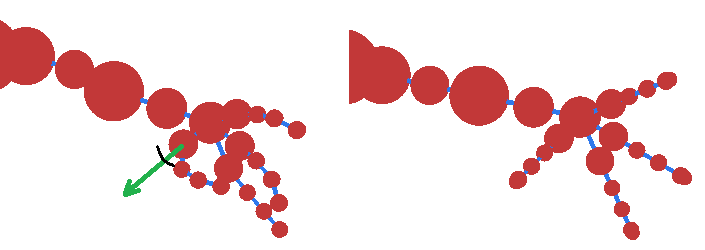
\includegraphics[width=\textwidth]{images/straightening2.png}
    \label{fig:straightening_ilu}
    \caption[Skeleton straightening]{Skeleton straightening; Left: input skeleton, green arrow represents the direction from connection nodes parents position to connection nodes position, black curve marks the distance between connection node and its child; Right: straightened skeleton}
\end{figure}

\subsection{Skinning matrices}
\paragraph{}
In final vertex placement we need to undo the rotations applied to the input skeleton during straightening. We have decided that the best solution is to use skinning, since it can be implemented on GPU and we wanted to move all post-processing on the GPU. Straightened skeleton represents bind pose for skinning purposes and the input skeleton represents reference pose. Now we can calculate skinning matrices required to transform bind pose to reference pose. Traditionally that would require to find the rotation between two corresponding nodes in respect to they parent. Rotating all child nodes in bind skeleton using the same rotation and propagate the rotation calculation to child nodes. But since we know precisely how bind pose was constructed, we can exploit this knowledge and avoid the rotation of child nodes. In fact we do not even need the bind skeleton itself.

\paragraph{}
This can be seen in Figure \ref{fig:DoF_estimation_ilu}. We want to calculate the rotation that would transform circle node to reference pose. We know that circle nodes parent square node is already in reference pose. We also know, that bind pose was constructed in such a way that all connection nodes childes are co-linear and preserve the distances between nodes. That means from squares reference pose we can calculate, where would be circle node, if we would apply on it the same transformation matrices as were applied to square node. The distance between square and circle node remains constant in both poses. And the direction at which the circle node would be is the same as the direction from triangle node to square node, which is marked as green arrow in Figure \ref{fig:DoF_estimation_ilu}. Now we only need to store the rotation between calculated circle node position, green circle in Figure \ref{fig:DoF_estimation_ilu} and its actual position red circle, with respect to its parent red square node.

\begin{figure}[h]
    \centering
    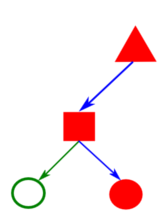
\includegraphics[]{images/DoF_estimation.png}
    \label{fig:DoF_estimation_ilu}
    \caption[Rotation estimation from reference pose]{Rotation estimation from reference pose. Circle: node which rotation we want to estimate; Square: parent of circle node; Triangle: parent of square node; Blue arrows: edges in reference pose; Green circle: circle node position after applying squares skinning matrices; Green arrow: direction from square to green circle node;}
\end{figure}

